\begin{figure}[H]
    \centering
    \begin{tabular}{p{5mm}*{4}{>{\centering\arraybackslash}p{1.15in}}c}
      \multirow[t]{5}{=}[-1in]{\rotatebox[origin=rc]{90}{Kitchen Scene}} & Ground Truth & CNN & CNN Mean Rescaled & CNN Histogram Matched & \\
      &
      \includegraphics[height=1.15in, width=1.15in]{captured/midas/8_29_kitchen_scene/gt_z_proj_crop_depth_fig.png}&
      \includegraphics[height=1.15in, width=1.15in]{captured/midas/8_29_kitchen_scene/z_init_depth_fig.png}&
      \includegraphics[height=1.15in, width=1.15in]{captured/midas/8_29_kitchen_scene/z_med_scaled_depth_fig.png}&
      \includegraphics[height=1.15in, width=1.15in]{captured/midas/8_29_kitchen_scene/z_pred_depth_fig.png}&
      \includegraphics[height=1.15in]{captured/midas/8_29_kitchen_scene/depth_colorbar.pdf}\\
%      & RGB &  &  &  & \\
      &
      \includegraphics[height=1.15in, width=1.15in]{captured/midas/8_29_kitchen_scene/rgb_cropped_fig.png}&
      \includegraphics[height=1.15in, width=1.15in]{captured/midas/8_29_kitchen_scene/z_init_diff_fig.png}&
      \includegraphics[height=1.15in, width=1.15in]{captured/midas/8_29_kitchen_scene/z_med_scaled_diff_fig.png}&
      \includegraphics[height=1.15in, width=1.15in]{captured/midas/8_29_kitchen_scene/z_pred_diff_fig.png}&
      \includegraphics[height=1.15in]{captured/midas/8_29_kitchen_scene/diff_colorbar.pdf}\\
      & RGB & RMSE = 2.914 & RMSE = 1.441 & RMSE = 0.606& \\ 

      \rule{0pt}{3ex}  & & & & & \\
      \multirow[t]{3}{=}{\rotatebox[origin=c]{90}{Conference Room 1}}& 
      \includegraphics[height=1.15in, width=1.15in]{captured/midas/8_29_conference_room_scene/gt_z_proj_crop_depth_fig.png}&
      \includegraphics[height=1.15in, width=1.15in]{captured/midas/8_29_conference_room_scene/z_init_depth_fig.png}&
      \includegraphics[height=1.15in, width=1.15in]{captured/midas/8_29_conference_room_scene/z_med_scaled_depth_fig.png}&
      \includegraphics[height=1.15in, width=1.15in]{captured/midas/8_29_conference_room_scene/z_pred_depth_fig.png}&
      \includegraphics[height=1.15in]{captured/midas/8_29_conference_room_scene/depth_colorbar.pdf}\\

      &
      \includegraphics[height=1.15in, width=1.15in]{captured/midas/8_29_conference_room_scene/rgb_cropped_fig.png}&
      \includegraphics[height=1.15in, width=1.15in]{captured/midas/8_29_conference_room_scene/z_init_diff_fig.png}&
      \includegraphics[height=1.15in, width=1.15in]{captured/midas/8_29_conference_room_scene/z_med_scaled_diff_fig.png}&
      \includegraphics[height=1.15in, width=1.15in]{captured/midas/8_29_conference_room_scene/z_pred_diff_fig.png}&
      \includegraphics[height=1.15in]{captured/midas/8_29_conference_room_scene/diff_colorbar.pdf}\\
      & & RMSE = 2.914 & RMSE = 1.441 & RMSE = 0.606& \\ 

      \rule{0pt}{3ex}  & & & & & \\
      \multirow[t]{3}{=}{\rotatebox[origin=c]{90}{Conference Room 2}}&
      \includegraphics[height=1.15in, width=1.15in]{captured/midas/8_30_conference_room2_scene/gt_z_proj_crop_depth_fig.png}&
      \includegraphics[height=1.15in, width=1.15in]{captured/midas/8_30_conference_room2_scene/z_init_depth_fig.png}&
      \includegraphics[height=1.15in, width=1.15in]{captured/midas/8_30_conference_room2_scene/z_med_scaled_depth_fig.png}&
      \includegraphics[height=1.15in, width=1.15in]{captured/midas/8_30_conference_room2_scene/z_pred_depth_fig.png}&
      \includegraphics[height=1.15in]{captured/midas/8_30_conference_room2_scene/depth_colorbar.pdf}\\

      &
      \includegraphics[height=1.15in, width=1.15in]{captured/midas/8_30_conference_room2_scene/rgb_cropped_fig.png}&
      \includegraphics[height=1.15in, width=1.15in]{captured/midas/8_30_conference_room2_scene/z_init_diff_fig.png}&
      \includegraphics[height=1.15in, width=1.15in]{captured/midas/8_30_conference_room2_scene/z_med_scaled_diff_fig.png}&
      \includegraphics[height=1.15in, width=1.15in]{captured/midas/8_30_conference_room2_scene/z_pred_diff_fig.png}&
      \includegraphics[height=1.15in]{captured/midas/8_30_conference_room2_scene/diff_colorbar.pdf}\\
      & & RMSE = 2.914 & RMSE = 1.441 & RMSE = 0.606& \\ 
    \end{tabular}
    \caption{Captured results initialized using the MiDaS CNN.
      Second row shows absolute difference between above estimates and ground
      truth. MiDaS does not output metric depth, so the CNN depth maps are
      scaled to be in the range $(0.494, 9.094)$ by default. However, MiDaS does produce
      accurate ordinal depth, leading to stronger performance of our histogram
      matching compared to other methods.}
    \label{fig:midas_captured_1}
%    \vspace{-1.5em}
\end{figure}
\begin{figure}[H]
    \centering
    \begin{tabular}{p{5mm}*{4}{>{\centering\arraybackslash}p{1.15in}}c}
      \multirow[t]{5}{=}[-1in]{\rotatebox[origin=rc]{90}{Hallway}} & Ground Truth & CNN & CNN Mean Rescaled & CNN Histogram Matched & \\
      &
      \includegraphics[width=1.15in, height=1.15in]{captured/midas/8_30_Hallway/gt_z_proj_crop_depth_fig.png}&
      \includegraphics[width=1.15in, height=1.15in]{captured/midas/8_30_Hallway/z_init_depth_fig.png}&
      \includegraphics[width=1.15in, height=1.15in]{captured/midas/8_30_Hallway/z_med_scaled_depth_fig.png}&
      \includegraphics[width=1.15in, height=1.15in]{captured/midas/8_30_Hallway/z_pred_depth_fig.png}&
      \includegraphics[height=1.15in]{captured/midas/8_30_Hallway/depth_colorbar.pdf}\\
      & & & & & \\

      & 
      \includegraphics[width=1.15in, height=1.15in]{captured/midas/8_30_Hallway/rgb_cropped_fig.png}&
      \includegraphics[width=1.15in, height=1.15in]{captured/midas/8_30_Hallway/z_init_diff_fig.png}&
      \includegraphics[width=1.15in, height=1.15in]{captured/midas/8_30_Hallway/z_med_scaled_diff_fig.png}&
      \includegraphics[width=1.15in, height=1.15in]{captured/midas/8_30_Hallway/z_pred_diff_fig.png}&
      \includegraphics[height=1.15in]{captured/midas/8_30_Hallway/diff_colorbar.pdf}\\
      & RGB & RMSE = 2.914 & RMSE = 1.441 & RMSE = 0.606& \\ 

      \rule{0pt}{3ex}  & & & & & \\
      \multirow[t]{3}{=}{\rotatebox[origin=c]{90}{Poster}}&
      \includegraphics[width=1.15in, height=1.15in]{captured/midas/8_30_poster_scene/gt_z_proj_crop_depth_fig.png}&
      \includegraphics[width=1.15in, height=1.15in]{captured/midas/8_30_poster_scene/z_init_depth_fig.png}&
      \includegraphics[width=1.15in, height=1.15in]{captured/midas/8_30_poster_scene/z_med_scaled_depth_fig.png}&
      \includegraphics[width=1.15in, height=1.15in]{captured/midas/8_30_poster_scene/z_pred_depth_fig.png}&
      \includegraphics[height=1.15in]{captured/midas/8_30_poster_scene/depth_colorbar.pdf}\\

      &
      \includegraphics[width=1.15in, height=1.15in]{captured/midas/8_30_poster_scene/rgb_cropped_fig.png}&
      \includegraphics[width=1.15in, height=1.15in]{captured/midas/8_30_poster_scene/z_init_diff_fig.png}&
      \includegraphics[width=1.15in, height=1.15in]{captured/midas/8_30_poster_scene/z_med_scaled_diff_fig.png}&
      \includegraphics[width=1.15in, height=1.15in]{captured/midas/8_30_poster_scene/z_pred_diff_fig.png}&
      \includegraphics[height=1.15in]{captured/midas/8_30_poster_scene/diff_colorbar.pdf}\\
      & & RMSE = 2.914 & RMSE = 1.441 & RMSE = 0.606& \\ 

      \rule{0pt}{3ex}  & & & & & \\
      \multirow[t]{3}{=}{\rotatebox[origin=c]{90}{Bookshelf}}&
      \includegraphics[width=1.15in, height=1.15in]{captured/midas/8_30_small_lab_scene/gt_z_proj_crop_depth_fig.png}&
      \includegraphics[width=1.15in, height=1.15in]{captured/midas/8_30_small_lab_scene/z_init_depth_fig.png}&
      \includegraphics[width=1.15in, height=1.15in]{captured/midas/8_30_small_lab_scene/z_med_scaled_depth_fig.png}&
      \includegraphics[width=1.15in, height=1.15in]{captured/midas/8_30_small_lab_scene/z_pred_depth_fig.png}&
      \includegraphics[height=1.15in]{captured/midas/8_30_small_lab_scene/depth_colorbar.pdf}\\

      &
      \includegraphics[width=1.15in, height=1.15in]{captured/midas/8_30_small_lab_scene/rgb_cropped_fig.png}&
      \includegraphics[width=1.15in, height=1.15in]{captured/midas/8_30_small_lab_scene/z_init_diff_fig.png}&
      \includegraphics[width=1.15in, height=1.15in]{captured/midas/8_30_small_lab_scene/z_med_scaled_diff_fig.png}&
      \includegraphics[width=1.15in, height=1.15in]{captured/midas/8_30_small_lab_scene/z_pred_diff_fig.png}&
      \includegraphics[height=1.15in]{captured/midas/8_30_small_lab_scene/diff_colorbar.pdf}\\
      & & RMSE = 2.914 & RMSE = 1.441 & RMSE = 0.606\\ 
                                     
%      (a)&(b)&(c)&(d)&(e)\\
    \end{tabular}
    \vspace{-1em}
    \caption{Captured results initialized using the MiDaS CNN.
      Second row shows absolute difference between above estimates and ground
      truth.MiDaS does not output metric depth, so the CNN depth maps are
      scaled to be in the range $(0.494, 9.094)$ by default. However, MiDaS does produce
      accurate ordinal depth, leading to stronger performance of our histogram
      matching compared to other methods.}
    \label{fig:midas_captured_2}
%    \vspace{-1.5em}
\end{figure}
 
% %% MiDaS outdoor scene
\begin{figure}[H]
    \centering
    \begin{tabular}{p{5mm}*{4}{>{\centering\arraybackslash}p{1.15in}}c}
      \multirow[t]{5}{=}[-1in]{\rotatebox[origin=rc]{90}{Outdoor Scene}} & Ground Truth & CNN & CNN Mean Rescaled & CNN Histogram Matched & \\
      &
      \includegraphics[height=1.15in, width=1.15in]{captured/midas/8_31_outdoor3/gt_z_proj_crop_depth_fig.png}&
      \includegraphics[height=1.15in, width=1.15in]{captured/midas/8_31_outdoor3/z_init_depth_fig.png}&
      \includegraphics[height=1.15in, width=1.15in]{captured/midas/8_31_outdoor3/z_med_scaled_depth_fig.png}&
      \includegraphics[height=1.15in, width=1.15in]{captured/midas/8_31_outdoor3/z_pred_depth_fig.png}&
      \includegraphics[height=1.15in]{captured/midas/8_31_outdoor3/depth_colorbar.pdf}\\
%      & RGB &  &  &  & \\
      &
      \includegraphics[height=1.15in, width=1.15in]{captured/midas/8_31_outdoor3/rgb_cropped_fig.png}&
      \includegraphics[height=1.15in, width=1.15in]{captured/midas/8_31_outdoor3/z_init_diff_fig.png}&
      \includegraphics[height=1.15in, width=1.15in]{captured/midas/8_31_outdoor3/z_med_scaled_diff_fig.png}&
      \includegraphics[height=1.15in, width=1.15in]{captured/midas/8_31_outdoor3/z_pred_diff_fig.png}&
      \includegraphics[height=1.15in]{captured/midas/8_31_outdoor3/diff_colorbar.pdf}\\
      & RGB & RMSE = 2.914 & RMSE = 1.441 & RMSE = 0.606& \\ 
    \end{tabular}
    \caption{Captured results initialized using the MiDaS CNN on an outdoor scene.
      Second row shows absolute difference between above estimates and ground
      truth. MiDaS does not output metric depth, so the CNN depth map is
      scaled to be in the range $(0.494, 11.094)$ by default. However, MiDaS does produce
      accurate ordinal depth, leading to stronger performance of our histogram
      matching compared to other methods.
}
    \label{fig:midas_captured_3}
%    \vspace{-1.5em}
\end{figure}


\begin{figure}[H]
    \centering
    \begin{tabular}{p{5mm}*{4}{>{\centering\arraybackslash}p{1.15in}}c}
      \multirow[t]{5}{=}[-1in]{\rotatebox[origin=rc]{90}{Kitchen Scene}} & Ground Truth & CNN & CNN Mean Rescaled & CNN Histogram Matched & \\
      &
      \includegraphics[height=1.15in, width=1.15in]{captured/densedepth/8_29_kitchen_scene/gt_z_proj_crop_depth_fig.png}&
      \includegraphics[height=1.15in, width=1.15in]{captured/densedepth/8_29_kitchen_scene/z_init_depth_fig.png}&
      \includegraphics[height=1.15in, width=1.15in]{captured/densedepth/8_29_kitchen_scene/z_med_scaled_depth_fig.png}&
      \includegraphics[height=1.15in, width=1.15in]{captured/densedepth/8_29_kitchen_scene/z_pred_depth_fig.png}&
      \includegraphics[height=1.15in]{captured/densedepth/8_29_kitchen_scene/depth_colorbar.pdf}\\
%      & RGB &  &  &  & \\
      &
      \includegraphics[height=1.15in, width=1.15in]{captured/densedepth/8_29_kitchen_scene/rgb_cropped_fig.png}&
      \includegraphics[height=1.15in, width=1.15in]{captured/densedepth/8_29_kitchen_scene/z_init_diff_fig.png}&
      \includegraphics[height=1.15in, width=1.15in]{captured/densedepth/8_29_kitchen_scene/z_med_scaled_diff_fig.png}&
      \includegraphics[height=1.15in, width=1.15in]{captured/densedepth/8_29_kitchen_scene/z_pred_diff_fig.png}&
      \includegraphics[height=1.15in]{captured/densedepth/8_29_kitchen_scene/diff_colorbar.pdf}\\
      & RGB & RMSE = 2.914 & RMSE = 1.441 & RMSE = 0.606& \\ 

      \rule{0pt}{3ex}  & & & & & \\
      \multirow[t]{3}{=}{\rotatebox[origin=c]{90}{Conference Room 1}}& 
      \includegraphics[height=1.15in, width=1.15in]{captured/densedepth/8_29_conference_room_scene/gt_z_proj_crop_depth_fig.png}&
      \includegraphics[height=1.15in, width=1.15in]{captured/densedepth/8_29_conference_room_scene/z_init_depth_fig.png}&
      \includegraphics[height=1.15in, width=1.15in]{captured/densedepth/8_29_conference_room_scene/z_med_scaled_depth_fig.png}&
      \includegraphics[height=1.15in, width=1.15in]{captured/densedepth/8_29_conference_room_scene/z_pred_depth_fig.png}&
      \includegraphics[height=1.15in]{captured/densedepth/8_29_conference_room_scene/depth_colorbar.pdf}\\

      &
      \includegraphics[height=1.15in, width=1.15in]{captured/densedepth/8_29_conference_room_scene/rgb_cropped_fig.png}&
      \includegraphics[height=1.15in, width=1.15in]{captured/densedepth/8_29_conference_room_scene/z_init_diff_fig.png}&
      \includegraphics[height=1.15in, width=1.15in]{captured/densedepth/8_29_conference_room_scene/z_med_scaled_diff_fig.png}&
      \includegraphics[height=1.15in, width=1.15in]{captured/densedepth/8_29_conference_room_scene/z_pred_diff_fig.png}&
      \includegraphics[height=1.15in]{captured/densedepth/8_29_conference_room_scene/diff_colorbar.pdf}\\
      & & RMSE = 2.914 & RMSE = 1.441 & RMSE = 0.606& \\ 

      \rule{0pt}{3ex}  & & & & & \\
      \multirow[t]{3}{=}{\rotatebox[origin=c]{90}{Conference Room 2}}&
      \includegraphics[height=1.15in, width=1.15in]{captured/densedepth/8_30_conference_room2_scene/gt_z_proj_crop_depth_fig.png}&
      \includegraphics[height=1.15in, width=1.15in]{captured/densedepth/8_30_conference_room2_scene/z_init_depth_fig.png}&
      \includegraphics[height=1.15in, width=1.15in]{captured/densedepth/8_30_conference_room2_scene/z_med_scaled_depth_fig.png}&
      \includegraphics[height=1.15in, width=1.15in]{captured/densedepth/8_30_conference_room2_scene/z_pred_depth_fig.png}&
      \includegraphics[height=1.15in]{captured/densedepth/8_30_conference_room2_scene/depth_colorbar.pdf}\\

      &
      \includegraphics[height=1.15in, width=1.15in]{captured/densedepth/8_30_conference_room2_scene/rgb_cropped_fig.png}&
      \includegraphics[height=1.15in, width=1.15in]{captured/densedepth/8_30_conference_room2_scene/z_init_diff_fig.png}&
      \includegraphics[height=1.15in, width=1.15in]{captured/densedepth/8_30_conference_room2_scene/z_med_scaled_diff_fig.png}&
      \includegraphics[height=1.15in, width=1.15in]{captured/densedepth/8_30_conference_room2_scene/z_pred_diff_fig.png}&
      \includegraphics[height=1.15in]{captured/densedepth/8_30_conference_room2_scene/diff_colorbar.pdf}\\
      & & RMSE = 2.914 & RMSE = 1.441 & RMSE = 0.606& \\ 
    \end{tabular}
    \caption{Captured results initialized using the DenseDepth CNN.
      Second row shows absolute difference between above estimates and ground truth.}
    \label{fig:densedepth_captured_1}
%    \vspace{-1.5em}
\end{figure}
\begin{figure}[H]
    \centering
    \begin{tabular}{p{5mm}*{4}{>{\centering\arraybackslash}p{1.15in}}c}
      \multirow[t]{5}{=}[-1in]{\rotatebox[origin=rc]{90}{Hallway}} & Ground Truth & CNN & CNN Mean Rescaled & CNN Histogram Matched & \\
      &
      \includegraphics[width=1.15in, height=1.15in]{captured/densedepth/8_30_Hallway/gt_z_proj_crop_depth_fig.png}&
      \includegraphics[width=1.15in, height=1.15in]{captured/densedepth/8_30_Hallway/z_init_depth_fig.png}&
      \includegraphics[width=1.15in, height=1.15in]{captured/densedepth/8_30_Hallway/z_med_scaled_depth_fig.png}&
      \includegraphics[width=1.15in, height=1.15in]{captured/densedepth/8_30_Hallway/z_pred_depth_fig.png}&
      \includegraphics[height=1.15in]{captured/densedepth/8_30_Hallway/depth_colorbar.pdf}\\
      & & & & & \\

      & 
      \includegraphics[width=1.15in, height=1.15in]{captured/densedepth/8_30_Hallway/rgb_cropped_fig.png}&
      \includegraphics[width=1.15in, height=1.15in]{captured/densedepth/8_30_Hallway/z_init_diff_fig.png}&
      \includegraphics[width=1.15in, height=1.15in]{captured/densedepth/8_30_Hallway/z_med_scaled_diff_fig.png}&
      \includegraphics[width=1.15in, height=1.15in]{captured/densedepth/8_30_Hallway/z_pred_diff_fig.png}&
      \includegraphics[height=1.15in]{captured/densedepth/8_30_Hallway/diff_colorbar.pdf}\\
      & RGB & RMSE = 2.914 & RMSE = 1.441 & RMSE = 0.606& \\ 

      \rule{0pt}{3ex}  & & & & & \\
      \multirow[t]{3}{=}{\rotatebox[origin=c]{90}{Poster}}&
      \includegraphics[width=1.15in, height=1.15in]{captured/densedepth/8_30_poster_scene/gt_z_proj_crop_depth_fig.png}&
      \includegraphics[width=1.15in, height=1.15in]{captured/densedepth/8_30_poster_scene/z_init_depth_fig.png}&
      \includegraphics[width=1.15in, height=1.15in]{captured/densedepth/8_30_poster_scene/z_med_scaled_depth_fig.png}&
      \includegraphics[width=1.15in, height=1.15in]{captured/densedepth/8_30_poster_scene/z_pred_depth_fig.png}&
      \includegraphics[height=1.15in]{captured/densedepth/8_30_poster_scene/depth_colorbar.pdf}\\

      &
      \includegraphics[width=1.15in, height=1.15in]{captured/densedepth/8_30_poster_scene/rgb_cropped_fig.png}&
      \includegraphics[width=1.15in, height=1.15in]{captured/densedepth/8_30_poster_scene/z_init_diff_fig.png}&
      \includegraphics[width=1.15in, height=1.15in]{captured/densedepth/8_30_poster_scene/z_med_scaled_diff_fig.png}&
      \includegraphics[width=1.15in, height=1.15in]{captured/densedepth/8_30_poster_scene/z_pred_diff_fig.png}&
      \includegraphics[height=1.15in]{captured/densedepth/8_30_poster_scene/diff_colorbar.pdf}\\
      & & RMSE = 2.914 & RMSE = 1.441 & RMSE = 0.606& \\ 

      \rule{0pt}{3ex}  & & & & & \\
      \multirow[t]{3}{=}{\rotatebox[origin=c]{90}{Bookshelf}}&
      \includegraphics[width=1.15in, height=1.15in]{captured/densedepth/8_30_small_lab_scene/gt_z_proj_crop_depth_fig.png}&
      \includegraphics[width=1.15in, height=1.15in]{captured/densedepth/8_30_small_lab_scene/z_init_depth_fig.png}&
      \includegraphics[width=1.15in, height=1.15in]{captured/densedepth/8_30_small_lab_scene/z_med_scaled_depth_fig.png}&
      \includegraphics[width=1.15in, height=1.15in]{captured/densedepth/8_30_small_lab_scene/z_pred_depth_fig.png}&
      \includegraphics[height=1.15in]{captured/densedepth/8_30_small_lab_scene/depth_colorbar.pdf}\\

      &
      \includegraphics[width=1.15in, height=1.15in]{captured/densedepth/8_30_small_lab_scene/rgb_cropped_fig.png}&
      \includegraphics[width=1.15in, height=1.15in]{captured/densedepth/8_30_small_lab_scene/z_init_diff_fig.png}&
      \includegraphics[width=1.15in, height=1.15in]{captured/densedepth/8_30_small_lab_scene/z_med_scaled_diff_fig.png}&
      \includegraphics[width=1.15in, height=1.15in]{captured/densedepth/8_30_small_lab_scene/z_pred_diff_fig.png}&
      \includegraphics[height=1.15in]{captured/densedepth/8_30_small_lab_scene/diff_colorbar.pdf}\\
      & & RMSE = 2.914 & RMSE = 1.441 & RMSE = 0.606\\ 
                                     
%      (a)&(b)&(c)&(d)&(e)\\
    \end{tabular}
    \caption{Captured results initialized using the DenseDepth CNN.
      Second row shows absolute difference between above estimates and ground truth.}
    \label{fig:densedepth_captured_2}
%    \vspace{-1.5em}
\end{figure}
%% DenseDepth outdoor scene
\begin{figure}[H]
    \centering
    \begin{tabular}{p{5mm}*{4}{>{\centering\arraybackslash}p{1.15in}}c}
      \multirow[t]{5}{=}[-1in]{\rotatebox[origin=rc]{90}{Outdoor Scene}} & Ground Truth & CNN & CNN Mean Rescaled & CNN Histogram Matched & \\
      &
      \includegraphics[height=1.15in, width=1.15in]{captured/densedepth/8_31_outdoor3/gt_z_proj_crop_depth_fig.png}&
      \includegraphics[height=1.15in, width=1.15in]{captured/densedepth/8_31_outdoor3/z_init_depth_fig.png}&
      \includegraphics[height=1.15in, width=1.15in]{captured/densedepth/8_31_outdoor3/z_med_scaled_depth_fig.png}&
      \includegraphics[height=1.15in, width=1.15in]{captured/densedepth/8_31_outdoor3/z_pred_depth_fig.png}&
      \includegraphics[height=1.15in]{captured/densedepth/8_31_outdoor3/depth_colorbar.pdf}\\
%      & RGB &  &  &  & \\
      &
      \includegraphics[height=1.15in, width=1.15in]{captured/densedepth/8_31_outdoor3/rgb_cropped_fig.png}&
      \includegraphics[height=1.15in, width=1.15in]{captured/densedepth/8_31_outdoor3/z_init_diff_fig.png}&
      \includegraphics[height=1.15in, width=1.15in]{captured/densedepth/8_31_outdoor3/z_med_scaled_diff_fig.png}&
      \includegraphics[height=1.15in, width=1.15in]{captured/densedepth/8_31_outdoor3/z_pred_diff_fig.png}&
      \includegraphics[height=1.15in]{captured/densedepth/8_31_outdoor3/diff_colorbar.pdf}\\
      & RGB & RMSE = 2.914 & RMSE = 1.441 & RMSE = 0.606& \\ 
    \end{tabular}
    \caption{Captured results initialized using the DenseDepth CNN on an outdoor scene.
      Second row shows absolute difference between above estimates and ground truth.}
    \label{fig:densedepth_captured_3}
%    \vspace{-1.5em}
\end{figure}


% %%%%%%%%%%%%%%%%%%%%%%%%%%%%%%%%%%%%%%%
 
\begin{figure}[H]
    \centering
    \begin{tabular}{p{5mm}*{4}{>{\centering\arraybackslash}p{1.15in}}c}
      \multirow[t]{5}{=}[-1in]{\rotatebox[origin=rc]{90}{Kitchen Scene}} & Ground Truth & CNN & CNN Mean Rescaled & CNN Histogram Matched & \\
      &
      \includegraphics[height=1.15in, width=1.15in]{captured/dorn/8_29_kitchen_scene/gt_z_proj_crop_depth_fig.png}&
      \includegraphics[height=1.15in, width=1.15in]{captured/dorn/8_29_kitchen_scene/z_init_depth_fig.png}&
      \includegraphics[height=1.15in, width=1.15in]{captured/dorn/8_29_kitchen_scene/z_med_scaled_depth_fig.png}&
      \includegraphics[height=1.15in, width=1.15in]{captured/dorn/8_29_kitchen_scene/z_pred_depth_fig.png}&
      \includegraphics[height=1.15in]{captured/dorn/8_29_kitchen_scene/depth_colorbar.pdf}\\
%      & RGB &  &  &  & \\
      &
      \includegraphics[height=1.15in, width=1.15in]{captured/dorn/8_29_kitchen_scene/rgb_cropped_fig.png}&
      \includegraphics[height=1.15in, width=1.15in]{captured/dorn/8_29_kitchen_scene/z_init_diff_fig.png}&
      \includegraphics[height=1.15in, width=1.15in]{captured/dorn/8_29_kitchen_scene/z_med_scaled_diff_fig.png}&
      \includegraphics[height=1.15in, width=1.15in]{captured/dorn/8_29_kitchen_scene/z_pred_diff_fig.png}&
      \includegraphics[height=1.15in]{captured/dorn/8_29_kitchen_scene/diff_colorbar.pdf}\\
      & RGB & RMSE = 2.914 & RMSE = 1.441 & RMSE = 0.606& \\ 

      \rule{0pt}{3ex}  & & & & & \\
      \multirow[t]{3}{=}{\rotatebox[origin=c]{90}{Conference Room 1}}& 
      \includegraphics[height=1.15in, width=1.15in]{captured/dorn/8_29_conference_room_scene/gt_z_proj_crop_depth_fig.png}&
      \includegraphics[height=1.15in, width=1.15in]{captured/dorn/8_29_conference_room_scene/z_init_depth_fig.png}&
      \includegraphics[height=1.15in, width=1.15in]{captured/dorn/8_29_conference_room_scene/z_med_scaled_depth_fig.png}&
      \includegraphics[height=1.15in, width=1.15in]{captured/dorn/8_29_conference_room_scene/z_pred_depth_fig.png}&
      \includegraphics[height=1.15in]{captured/dorn/8_29_conference_room_scene/depth_colorbar.pdf}\\

      &
      \includegraphics[height=1.15in, width=1.15in]{captured/dorn/8_29_conference_room_scene/rgb_cropped_fig.png}&
      \includegraphics[height=1.15in, width=1.15in]{captured/dorn/8_29_conference_room_scene/z_init_diff_fig.png}&
      \includegraphics[height=1.15in, width=1.15in]{captured/dorn/8_29_conference_room_scene/z_med_scaled_diff_fig.png}&
      \includegraphics[height=1.15in, width=1.15in]{captured/dorn/8_29_conference_room_scene/z_pred_diff_fig.png}&
      \includegraphics[height=1.15in]{captured/dorn/8_29_conference_room_scene/diff_colorbar.pdf}\\
      & & RMSE = 2.914 & RMSE = 1.441 & RMSE = 0.606& \\ 

      \rule{0pt}{3ex}  & & & & & \\
      \multirow[t]{3}{=}{\rotatebox[origin=c]{90}{Conference Room 2}}&
      \includegraphics[height=1.15in, width=1.15in]{captured/dorn/8_30_conference_room2_scene/gt_z_proj_crop_depth_fig.png}&
      \includegraphics[height=1.15in, width=1.15in]{captured/dorn/8_30_conference_room2_scene/z_init_depth_fig.png}&
      \includegraphics[height=1.15in, width=1.15in]{captured/dorn/8_30_conference_room2_scene/z_med_scaled_depth_fig.png}&
      \includegraphics[height=1.15in, width=1.15in]{captured/dorn/8_30_conference_room2_scene/z_pred_depth_fig.png}&
      \includegraphics[height=1.15in]{captured/dorn/8_30_conference_room2_scene/depth_colorbar.pdf}\\

      &
      \includegraphics[height=1.15in, width=1.15in]{captured/dorn/8_30_conference_room2_scene/rgb_cropped_fig.png}&
      \includegraphics[height=1.15in, width=1.15in]{captured/dorn/8_30_conference_room2_scene/z_init_diff_fig.png}&
      \includegraphics[height=1.15in, width=1.15in]{captured/dorn/8_30_conference_room2_scene/z_med_scaled_diff_fig.png}&
      \includegraphics[height=1.15in, width=1.15in]{captured/dorn/8_30_conference_room2_scene/z_pred_diff_fig.png}&
      \includegraphics[height=1.15in]{captured/dorn/8_30_conference_room2_scene/diff_colorbar.pdf}\\
      & & RMSE = 2.914 & RMSE = 1.441 & RMSE = 0.606& \\ 
    \end{tabular}
    \caption{Captured results initialized using the DORN CNN.
      Second row shows absolute difference between above estimates and ground truth.}
    \label{fig:dorn_captured_1}
%    \vspace{-1.5em}
\end{figure}

\begin{figure}[H]
    \centering
    \begin{tabular}{p{5mm}*{4}{>{\centering\arraybackslash}p{1.15in}}c}
      \multirow[t]{5}{=}[-1in]{\rotatebox[origin=rc]{90}{Hallway}} & Ground Truth & CNN & CNN Mean Rescaled & CNN Histogram Matched & \\
      &
      \includegraphics[width=1.15in, height=1.15in]{captured/dorn/8_30_Hallway/gt_z_proj_crop_depth_fig.png}&
      \includegraphics[width=1.15in, height=1.15in]{captured/dorn/8_30_Hallway/z_init_depth_fig.png}&
      \includegraphics[width=1.15in, height=1.15in]{captured/dorn/8_30_Hallway/z_med_scaled_depth_fig.png}&
      \includegraphics[width=1.15in, height=1.15in]{captured/dorn/8_30_Hallway/z_pred_depth_fig.png}&
      \includegraphics[height=1.15in]{captured/dorn/8_30_Hallway/depth_colorbar.pdf}\\
      & & & & & \\

      & 
      \includegraphics[width=1.15in, height=1.15in]{captured/dorn/8_30_Hallway/rgb_cropped_fig.png}&
      \includegraphics[width=1.15in, height=1.15in]{captured/dorn/8_30_Hallway/z_init_diff_fig.png}&
      \includegraphics[width=1.15in, height=1.15in]{captured/dorn/8_30_Hallway/z_med_scaled_diff_fig.png}&
      \includegraphics[width=1.15in, height=1.15in]{captured/dorn/8_30_Hallway/z_pred_diff_fig.png}&
      \includegraphics[height=1.15in]{captured/dorn/8_30_Hallway/diff_colorbar.pdf}\\
      & RGB & RMSE = 2.914 & RMSE = 1.441 & RMSE = 0.606& \\ 

      \rule{0pt}{3ex}  & & & & & \\
      \multirow[t]{3}{=}{\rotatebox[origin=c]{90}{Poster}}&
      \includegraphics[width=1.15in, height=1.15in]{captured/dorn/8_30_poster_scene/gt_z_proj_crop_depth_fig.png}&
      \includegraphics[width=1.15in, height=1.15in]{captured/dorn/8_30_poster_scene/z_init_depth_fig.png}&
      \includegraphics[width=1.15in, height=1.15in]{captured/dorn/8_30_poster_scene/z_med_scaled_depth_fig.png}&
      \includegraphics[width=1.15in, height=1.15in]{captured/dorn/8_30_poster_scene/z_pred_depth_fig.png}&
      \includegraphics[height=1.15in]{captured/dorn/8_30_poster_scene/depth_colorbar.pdf}\\

      &
      \includegraphics[width=1.15in, height=1.15in]{captured/dorn/8_30_poster_scene/rgb_cropped_fig.png}&
      \includegraphics[width=1.15in, height=1.15in]{captured/dorn/8_30_poster_scene/z_init_diff_fig.png}&
      \includegraphics[width=1.15in, height=1.15in]{captured/dorn/8_30_poster_scene/z_med_scaled_diff_fig.png}&
      \includegraphics[width=1.15in, height=1.15in]{captured/dorn/8_30_poster_scene/z_pred_diff_fig.png}&
      \includegraphics[height=1.15in]{captured/dorn/8_30_poster_scene/diff_colorbar.pdf}\\
      & & RMSE = 2.914 & RMSE = 1.441 & RMSE = 0.606& \\ 

      \rule{0pt}{3ex}  & & & & & \\
      \multirow[t]{3}{=}{\rotatebox[origin=c]{90}{Bookshelf}}&
      \includegraphics[width=1.15in, height=1.15in]{captured/dorn/8_30_small_lab_scene/gt_z_proj_crop_depth_fig.png}&
      \includegraphics[width=1.15in, height=1.15in]{captured/dorn/8_30_small_lab_scene/z_init_depth_fig.png}&
      \includegraphics[width=1.15in, height=1.15in]{captured/dorn/8_30_small_lab_scene/z_med_scaled_depth_fig.png}&
      \includegraphics[width=1.15in, height=1.15in]{captured/dorn/8_30_small_lab_scene/z_pred_depth_fig.png}&
      \includegraphics[height=1.15in]{captured/dorn/8_30_small_lab_scene/depth_colorbar.pdf}\\

      &
      \includegraphics[width=1.15in, height=1.15in]{captured/dorn/8_30_small_lab_scene/rgb_cropped_fig.png}&
      \includegraphics[width=1.15in, height=1.15in]{captured/dorn/8_30_small_lab_scene/z_init_diff_fig.png}&
      \includegraphics[width=1.15in, height=1.15in]{captured/dorn/8_30_small_lab_scene/z_med_scaled_diff_fig.png}&
      \includegraphics[width=1.15in, height=1.15in]{captured/dorn/8_30_small_lab_scene/z_pred_diff_fig.png}&
      \includegraphics[height=1.15in]{captured/dorn/8_30_small_lab_scene/diff_colorbar.pdf}\\
      & & RMSE = 2.914 & RMSE = 1.441 & RMSE = 0.606\\ 
                                     
%      (a)&(b)&(c)&(d)&(e)\\
    \end{tabular}
    \caption{Captured results initialized using the DORN CNN.
      Second row shows absolute difference between above estimates and ground truth.}
    \label{fig:dorn_captured_2}
%    \vspace{-1.5em}
\end{figure}
% %% DORN outdoor scene
% \begin{figure}
%     \centering
%     \begin{tabular}{p{5mm}*{4}{>{\centering\arraybackslash}p{1.15in}}c}
%       \multirow[t]{5}{=}[-1in]{\rotatebox[origin=rc]{90}{Outdoor Scene}} & Ground Truth & CNN & CNN Mean Rescaled & CNN Histogram Matched & \\
%       &
%       \includegraphics[height=1.15in, width=1.15in]{captured/dorn/8_31_outdoor3/gt_z_proj_crop_depth_fig.png}&
%       \includegraphics[height=1.15in, width=1.15in]{captured/dorn/8_31_outdoor3/z_init_depth_fig.png}&
%       \includegraphics[height=1.15in, width=1.15in]{captured/dorn/8_31_outdoor3/z_med_scaled_depth_fig.png}&
%       \includegraphics[height=1.15in, width=1.15in]{captured/dorn/8_31_outdoor3/z_pred_depth_fig.png}&
%       \includegraphics[height=1.15in]{captured/dorn/8_31_outdoor3/depth_colorbar.pdf}\\
% %      & RGB &  &  &  & \\
%       &
%       \includegraphics[height=1.15in, width=1.15in]{captured/dorn/8_31_outdoor3/rgb_cropped_fig.png}&
%       \includegraphics[height=1.15in, width=1.15in]{captured/dorn/8_31_outdoor3/z_init_diff_fig.png}&
%       \includegraphics[height=1.15in, width=1.15in]{captured/dorn/8_31_outdoor3/z_med_scaled_diff_fig.png}&
%       \includegraphics[height=1.15in, width=1.15in]{captured/dorn/8_31_outdoor3/z_pred_diff_fig.png}&
%       \includegraphics[height=1.15in]{captured/dorn/8_31_outdoor3/diff_colorbar.pdf}\\
%       & RGB & RMSE = 2.914 & RMSE = 1.441 & RMSE = 0.606& \\ 
%     \end{tabular}
%     \caption{Captured results initialized using the DORN CNN on an outdoor scene.
%       Second row shows absolute difference between above estimates and ground truth.}
%     \label{fig:dorn_outdoor_captured}
% %    \vspace{-1.5em}
% \end{figure}

\begin{figure}[H]
    \centering
    \begin{tabular}{p{5mm}*{4}{>{\centering\arraybackslash}p{1.15in}}c}
      \multirow[t]{5}{=}[-1in]{\rotatebox[origin=rc]{90}{Outdoor Scene}} & Ground Truth & CNN & CNN Mean Rescaled & CNN Histogram Matched & \\
      &
      \includegraphics[height=1.15in, width=1.15in]{captured/dorn/8_31_outdoor3/gt_z_proj_crop_depth_fig.png}&
      \includegraphics[height=1.15in, width=1.15in]{captured/dorn/8_31_outdoor3/z_init_depth_fig.png}&
      \includegraphics[height=1.15in, width=1.15in]{captured/dorn/8_31_outdoor3/z_med_scaled_depth_fig.png}&
      \includegraphics[height=1.15in, width=1.15in]{captured/dorn/8_31_outdoor3/z_pred_depth_fig.png}&
      \includegraphics[height=1.15in]{captured/dorn/8_31_outdoor3/depth_colorbar.pdf}\\
%      & RGB &  &  &  & \\
      &
      \includegraphics[height=1.15in, width=1.15in]{captured/dorn/8_31_outdoor3/rgb_cropped_fig.png}&
      \includegraphics[height=1.15in, width=1.15in]{captured/dorn/8_31_outdoor3/z_init_diff_fig.png}&
      \includegraphics[height=1.15in, width=1.15in]{captured/dorn/8_31_outdoor3/z_med_scaled_diff_fig.png}&
      \includegraphics[height=1.15in, width=1.15in]{captured/dorn/8_31_outdoor3/z_pred_diff_fig.png}&
      \includegraphics[height=1.15in]{captured/dorn/8_31_outdoor3/diff_colorbar.pdf}\\
      & RGB & RMSE = 2.914 & RMSE = 1.441 & RMSE = 0.606& \\ 
    \end{tabular}
    \caption{Captured results initialized using the DORN CNN on an outdoor scene.
      Second row shows absolute difference between above estimates and ground truth.}
    \label{fig:dorn_captured_3}
%    \vspace{-1.5em}
\end{figure}

